\chapter{超音速牛奶喷射与时间旅行的异构关系}

本章在前两章模型的基础上讨论两个子系统之间的耦合关系。这里的数字和图形只用于演示论文写作结构，不代表真实实验结论；正式论文应把示例数据替换为可复现的实验记录，并在图题或正文中说明数据来源。

\section{综合分析框架}

\subsection{喷射过程与时间参数的耦合}

喷射状态可以用速度、密度和喷嘴几何参数描述，时间状态则用离散的观测时刻与转移概率描述。为了避免把两个模型简单相加，本研究将它们放入同一状态空间，并以耦合系数控制信息从喷射子系统向时间子系统的传递。这样的建模方式有两个优点：一是能够明确区分直接观测量与隐变量，二是方便在后续敏感性分析中逐一关闭耦合项。

\subsection{模型假设与评价指标}

综合模型假设观测误差在相邻时间窗内近似独立，且喷射效率可以由无量纲速度、压力比和状态转移概率共同解释。评价时同时报告均方误差、置信区间和状态转移成功率，避免仅凭一条拟合曲线判断模型优劣。对于实际研究，还需要补充采样频率、异常值处理和训练/验证集划分。

\subsection{结构关系图}

图~\ref{fig:structure-relations}说明数据、模型和预测结果之间的依赖关系。箭头表示方向，节点颜色承担分组功能；这种表达适合在黑白打印时保持关系清楚。
\begin{figure}[htbp]
  \centering
  \begin{tikzpicture}[>=Stealth,node distance=14mm,
    block/.style={draw,rounded corners,minimum width=32mm,minimum height=12mm,align=center}]
    \node[block,fill=blue!7] (obs) {观测数据};
    \node[block,fill=teal!7,right=of obs] (model) {概率模型};
    \node[block,fill=yellow!12,right=of model] (pred) {预测结果};
    \draw[-{Stealth},thick] (obs)--(model);
    \draw[-{Stealth},thick] (model)--(pred);
  \end{tikzpicture}
  \caption{综合模型的结构关系图}
  \label{fig:structure-relations}
\end{figure}

图~\ref{fig:structure-relations}不是结果图，而是帮助读者理解变量之间的依赖方向。正文在引用示意图时应解释图中关系与后续公式的对应位置，避免只在段末写“如图所示”。

\section{模拟结果}

\subsection{参数响应曲线}

为说明数据绘图在正文中的表达方式，图~\ref{fig:response-comparison}用一组小型模拟数据比较观测值和模型响应。图题、编号、上下间距和页眉页脚由论文模板统一处理。
\begin{figure}[htbp]
  \centering
  \begin{tikzpicture}
    \begin{axis}[
      width=.78\textwidth,height=5.3cm,
      xmin=0,xmax=6.2,ymin=.25,ymax=.9,
      xtick={0,1,2,3,4,5,6},ytick={.3,.4,.5,.6,.7,.8},
      xlabel={$t$},ylabel={$P(t)$},grid=major,
      grid style={black!12,line width=.35pt},
      tick label style={font=\scriptsize},label style={font=\small},
      legend style={draw=none,font=\scriptsize,at={(.5,-.22)},anchor=north,legend columns=2}]
      \addplot+[only marks,black,mark=*,mark size=1.4pt]
        coordinates {(0,.48)(1,.62)(2,.74)(3,.69)(4,.58)(5,.46)(6,.38)};
      \addlegendentry{观测值}
      \addplot+[no markers,black,line width=.8pt,smooth]
        coordinates {(0,.50)(1,.7919)(2,.5735)(3,.3583)(4,.4240)(5,.5587)(6,.5565)};
      \addlegendentry{模型响应}
    \end{axis}
  \end{tikzpicture}
  \caption{观测值与模型响应的比较（模拟数据）}
  \label{fig:response-comparison}
\end{figure}

从图~\ref{fig:response-comparison}可见，示例模型在中间时段的响应与观测值存在明显差异，后续分析应结合参数区间、残差图和边界条件判断误差来源。由于数据是模拟的，这张图只展示结果段的表达方式，不支持对真实装置性能的结论。

为便于检查数据表达的一致性，图~\ref{fig:response-curve}再次展示相同的观测值与模型响应。图中散点对应观测值，实线对应模型响应，坐标轴标签和图例采用与正文一致的符号体系。
\begin{figure}[htbp]
  \centering
  \begin{tikzpicture}
    \begin{axis}[
      width=.78\textwidth,height=5.3cm,
      xmin=0,xmax=6.2,ymin=.25,ymax=.9,
      xtick={0,1,2,3,4,5,6},ytick={.3,.4,.5,.6,.7,.8},
      xlabel={$t$},ylabel={$P(t)$},grid=major,
      grid style={black!12,line width=.35pt},
      tick label style={font=\scriptsize},label style={font=\small},
      legend style={draw=none,font=\scriptsize,at={(.5,-.22)},anchor=north,legend columns=2}]
      \addplot+[only marks,black,mark=*,mark size=1.4pt]
        coordinates {(0,.48)(1,.62)(2,.74)(3,.69)(4,.58)(5,.46)(6,.38)};
      \addlegendentry{观测值}
      \addplot+[no markers,black,line width=.8pt,smooth]
        coordinates {(0,.50)(1,.7919)(2,.5735)(3,.3583)(4,.4240)(5,.5587)(6,.5565)};
      \addlegendentry{模型响应}
    \end{axis}
  \end{tikzpicture}
  \caption{观测值与模型响应曲线（模拟数据）}
  \label{fig:response-curve}
\end{figure}

图形中应保持字体、字号和线宽一致，并在图注中说明数据来源与处理方法。

图~\ref{fig:diagnostics-panel}并列展示三维曲面、局部向量场、矩阵色图和极坐标响应，分别用于观察标量场形态、局部方向、离散网格分布和角向变化。这些示例采用模拟数据，正式研究中应替换为可追溯的实验或仿真结果，并说明变量定义和数据处理过程。
\begin{figure}[htbp]
  \centering
  % PGFPlots surface, vector-field, matrix, and polar panels as subfigures.
\begin{subfigure}[t]{0.48\textwidth}
  \centering
  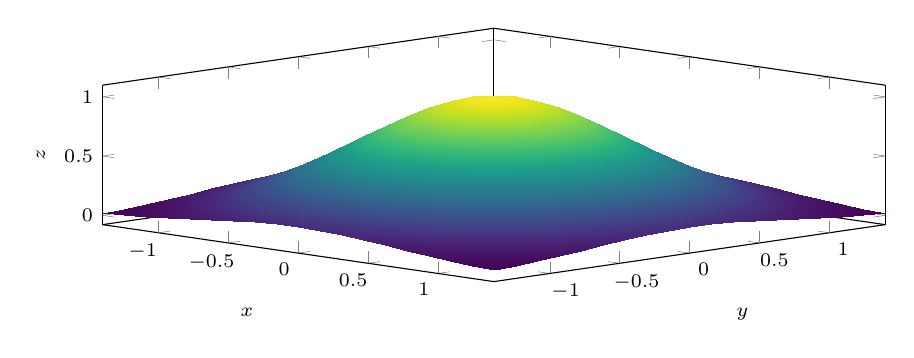
\begin{tikzpicture}
    \begin{axis}[
      width=.95\linewidth,height=48mm,
      tick label style={font=\scriptsize},label style={font=\scriptsize},
      view={45}{30},xlabel={$x$},ylabel={$y$},zlabel={$z$},
      colormap/viridis,domain=-1.4:1.4,y domain=-1.4:1.4]
      \addplot3[surf,shader=interp,samples=19,samples y=19] {exp(-x^2-y^2)};
    \end{axis}
  \end{tikzpicture}
  \caption{三维曲面}
\end{subfigure}\hfill
\begin{subfigure}[t]{0.48\textwidth}
  \centering
  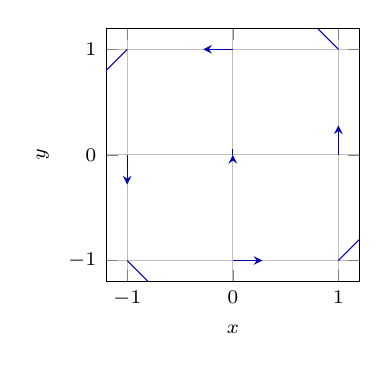
\begin{tikzpicture}
    \begin{axis}[
      width=.95\linewidth,height=48mm,
      tick label style={font=\scriptsize},label style={font=\scriptsize},
      xlabel={$x$},ylabel={$y$},xmin=-1.2,xmax=1.2,ymin=-1.2,ymax=1.2,
      axis equal image,grid=major]
      \addplot[blue!70!black,-stealth,
        quiver={u=\thisrow{u},v=\thisrow{v},scale arrows=.28}] table[row sep=crcr] {
        x y u v\\
        -1 -1 1 -1\\
         0 -1 1  0\\
         1 -1 1  1\\
        -1  0 0 -1\\
         0  0 0  0\\
         1  0 0  1\\
        -1  1 -1 -1\\
         0  1 -1  0\\
         1  1 -1  1\\
      };
    \end{axis}
  \end{tikzpicture}
  \caption{局部向量场}
\end{subfigure}

\par\medskip

\begin{subfigure}[t]{0.48\textwidth}
  \centering
  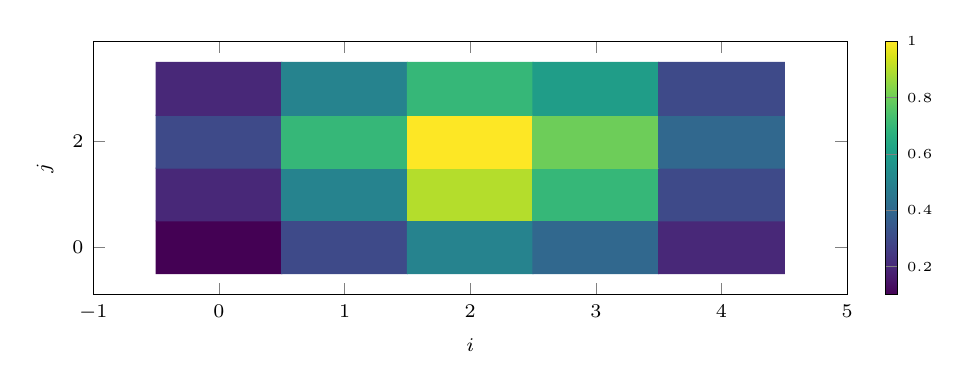
\begin{tikzpicture}
    \begin{axis}[
      tick label style={font=\scriptsize},label style={font=\scriptsize},
      width=.92\linewidth,height=48mm,
      xlabel={$i$},ylabel={$j$},view={0}{90},colorbar,colormap/viridis,
      colorbar style={width=1.5mm,tick label style={font=\tiny}}]
      \addplot[matrix plot*,mesh/cols=5,point meta=explicit] table[meta=z,row sep=crcr] {
        x y z\\
        0 0 .1\\ 1 0 .3\\ 2 0 .5\\ 3 0 .4\\ 4 0 .2\\
        0 1 .2\\ 1 1 .5\\ 2 1 .9\\ 3 1 .7\\ 4 1 .3\\
        0 2 .3\\ 1 2 .7\\ 2 2 1.0\\ 3 2 .8\\ 4 2 .4\\
        0 3 .2\\ 1 3 .5\\ 2 3 .7\\ 3 3 .6\\ 4 3 .3\\
      };
    \end{axis}
  \end{tikzpicture}
  \caption{矩阵色图}
\end{subfigure}\hfill
\begin{subfigure}[t]{0.48\textwidth}
  \centering
  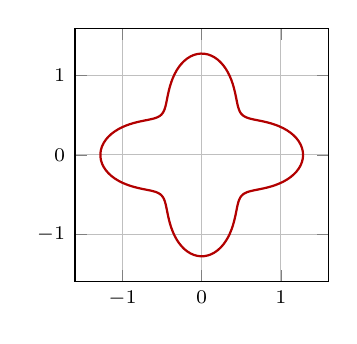
\begin{tikzpicture}
    \begin{axis}[
      width=.95\linewidth,height=48mm,
      tick label style={font=\scriptsize},label style={font=\scriptsize},
      axis equal image,grid=major,xmin=-1.6,xmax=1.6,ymin=-1.6,ymax=1.6]
      \addplot[red!70!black,thick,domain=0:360,samples=180]
        ({(1+.28*cos(4*x))*cos(x)},{(1+.28*cos(4*x))*sin(x)});
    \end{axis}
  \end{tikzpicture}
  \caption{极坐标响应}
\end{subfigure}

  \caption{多类型数值图形示例组}
  \label{fig:diagnostics-panel}
\end{figure}

\subsection{多视图结果组织示例}

为对照模型响应、残差变化、离散误差和区间覆盖率，图~\ref{fig:response-multipanel}将四种结果视图放在同一组中。图中数据为排版示例，正式分析应报告数据来源、样本规模和计算设置，并结合相应指标讨论模型表现。
\begin{figure}[htbp]
  \centering
  % Adapted PGFPlots group-plot example for response, residual, convergence, and coverage.
\begin{tikzpicture}
  \begin{groupplot}[
    group style={group size=2 by 2,horizontal sep=11mm,vertical sep=15mm},
    width=61mm,height=30mm,
    tick label style={font=\scriptsize},label style={font=\scriptsize},
    title style={font=\small},grid=major,grid style={black!12},
  ]
    \nextgroupplot[title={观测与模型响应},xlabel={$t$},ylabel={$P(t)$},
      xmin=0,xmax=6,ymin=.2,ymax=.9]
      \addplot+[only marks,black,mark=*,error bars/.cd,y dir=both,y explicit]
        coordinates {(0,.48)+-(0,.04) (1,.62)+-(0,.05) (2,.74)+-(0,.04)
          (3,.69)+-(0,.05) (4,.58)+-(0,.04) (5,.46)+-(0,.04) (6,.38)+-(0,.03)};
      \addplot+[blue!70!black,thick,no markers,smooth]
        coordinates {(0,.50) (1,.60) (2,.70) (3,.67) (4,.57) (5,.45) (6,.39)};

    \nextgroupplot[title={残差随时间变化},xlabel={$t$},ylabel={$e(t)$},
      xmin=0,xmax=6,ymin=-.2,ymax=.2]
      \addplot+[only marks,teal!70!black,mark=square*]
        coordinates {(0,-.02) (1,.04) (2,.09) (3,.02) (4,-.03) (5,.01) (6,-.01)};
      \addplot[black,dashed,no markers,domain=0:6] {0};

    \nextgroupplot[title={离散误差收敛},xlabel={$h$},ylabel={误差},
      xmode=log,ymode=log,xmin=.08,xmax=1.1,ymin=.001,ymax=.5,
      log ticks with fixed point,
      xtick={1,.5,.25,.125},ytick={.1,.01,.001},
      xticklabel style={/pgf/number format/fixed,/pgf/number format/precision=3}]
      \addplot+[mark=*,blue!70!black,thick] coordinates
        {(1,.32) (.5,.081) (.25,.020) (.125,.0051)};
      \addplot+[black,dashed,no markers,domain=.1:1,samples=40] {0.32*x^2};

    \nextgroupplot[title={区间覆盖率},xlabel={样本量},ylabel={覆盖率},
      xmin=100,xmax=1000,ymin=.82,ymax=1.0,xtick={100,400,700,1000}]
      \addplot+[only marks,mark=triangle*,orange!80!black]
        coordinates {(100,.89) (250,.92) (400,.95) (600,.94) (800,.96) (1000,.95)};
      \addplot[black,dashed,no markers,domain=100:1000] {.95};
  \end{groupplot}
\end{tikzpicture}

  \caption{响应、误差和覆盖率的多视图图组}
  \label{fig:response-multipanel}
\end{figure}

\section{数值离散与误差分析}

\subsection{空间与时间离散}

把连续的输运方程交给计算机求解，第一步是把导数换成差分。中心差分在相同网格下比单侧差分高一阶，代价是需要相邻两个网格点的值，因此在边界附近必须降阶处理。
\begin{equation}
  \left.\frac{\partial u}{\partial x}\right|_i
  \approx\frac{u_{i+1}-u_i}{h}+O(h),\qquad
  \left.\frac{\partial u}{\partial x}\right|_i
  \approx\frac{u_{i+1}-u_{i-1}}{2h}+O(h^2).
  \label{eq:fd-stencils}
\end{equation}
\begin{equation}
  \left.\frac{\partial^2u}{\partial x^2}\right|_i
  \approx\frac{u_{i+1}-2u_i+u_{i-1}}{h^2}+O(h^2).
  \label{eq:fd-stencil-second}
\end{equation}

时间方向可以显式推进，也可以隐式求解。显式格式每步只做一次函数求值，但受步长限制；隐式格式每步要解一个线性方程组，换来了更大的稳定域。
\begin{equation}
  \bm{u}^{n+1}=\bm{u}^{n}+\Delta t\,\bm{F}(\bm{u}^{n}),\qquad
  (\bm{I}-\Delta t\,\bm{J})\bm{u}^{n+1}
    =\bm{u}^{n}+\Delta t\,\bm{g},\qquad
  \bm{J}=\frac{\partial\bm{F}}{\partial\bm{u}}.
  \label{eq:time-stepping}
\end{equation}

把显式和隐式加权组合可以得到二阶精度的 Crank--Nicolson 格式。权重取 $1/2$ 时截断误差的主项相互抵消，但每步的计算量与隐式格式相同。
\begin{equation}
  \frac{\bm{u}^{n+1}-\bm{u}^{n}}{\Delta t}
  =\frac{1}{2}\left[\bm{F}(\bm{u}^{n+1})+\bm{F}(\bm{u}^{n})\right].
  \label{eq:crank-nicolson}
\end{equation}

\subsection{截断误差与收敛阶}

误差随步长下降的速度决定了加密网格的收益。若误差按 $h^p$ 下降，则步长减半时期望误差降为原来的 $2^{-p}$；实测阶数可以用两次不同步长的结果反算，并用于检查实现是否正确。
\begin{equation}
  e_h=\|\bm{u}_h-\bm{u}\|=Ch^p+O(h^{p+1}),\qquad
  p=\log_2\left(\frac{e_h}{e_{h/2}}\right).
  \label{eq:convergence-order}
\end{equation}

已知误差的主项形状后，可以用两个不同步长的解消去主项，得到更高精度的外推结果。这一技巧在网格序列收敛性验证中比单纯加密网格更经济。
\begin{equation}
  \tilde{u}_h=\frac{2^p u_{h/2}-u_h}{2^p-1}.
  \label{eq:richardson}
\end{equation}
\begin{equation}
  e_{\mathrm{total}}
  =\underbrace{e_{\mathrm{trunc}}}_{\text{格式}}
  +\underbrace{e_{\mathrm{round}}}_{\text{字长}}
  +\underbrace{e_{\mathrm{model}}}_{\text{假设}}.
  \label{eq:error-sources}
\end{equation}

\subsection{稳定性与步长约束}

显式格式的步长受网格尺度和物理系数共同限制。扩散项的时间步长与空间步长的平方成正比，对流项则与空间步长成正比，因此细网格下扩散往往成为限制因素。
\begin{equation}
  \Delta t\leq\frac{h^2}{2D},\qquad
  \Delta t\leq\frac{h}{|v|_{\max}},\qquad
  \mathrm{CFL}=\frac{|v|\Delta t}{h}\leq1.
  \label{eq:cfl}
\end{equation}

稳定性的频域判据把放大因子写成波数和步长的函数。要求放大因子的模不超过 1，就得到与上面一致的步长约束。
\begin{equation}
  |g(\vartheta)|\leq1,\quad \vartheta\in[0,\pi],\qquad
  g(\vartheta)=1-4\nu\sin^2(\vartheta/2),\quad
  \nu=\frac{D\Delta t}{h^2}.
  \label{eq:von-neumann}
\end{equation}

表~\ref{tab:schemes}对比常用离散格式的精度与代价。表中代价按每步的函数求值次数和线性求解次数给出，不含数据读写。
\begin{table}[htbp]
  \centering
  \caption{常用离散格式的精度、稳定性与代价对照}
  \label{tab:schemes}
  \small
  \begin{tabularx}{\textwidth}{>{\centering\arraybackslash}p{0.16\textwidth}>{\centering\arraybackslash}p{0.13\textwidth}>{\centering\arraybackslash}X>{\centering\arraybackslash}X>{\centering\arraybackslash}X}
    \toprule
    \textbf{格式} & \textbf{时间精度} & \textbf{稳定性} & \textbf{每步代价} & \textbf{适用场景}\\
    \midrule
    显式欧拉 & 一阶 & 需满足步长限制 & 一次函数求值 & 短时、刚性弱\\
    隐式欧拉 & 一阶 & 无条件稳定 & 一次线性求解 & 刚性、长时\\
    Crank--Nicolson & 二阶 & 对扩散问题无条件稳定 & 一次线性求解 & 扩散主导\\
    四阶 Runge--Kutta & 四阶 & 步长限制较宽 & 四次函数求值 & 光滑非刚性\\
    \bottomrule
  \end{tabularx}
\end{table}

\subsection{参数扫描与转页长表}

参数扫描会得到行数较多的结果表。跨页表格应在续页重复表头，读者不必回到上一页寻找列名。表~\ref{tab:sweep}的行数用于展示长表编排，数值为排版示例，不是计算记录。
\begin{small}
\begin{longtable}{@{}c c c c c c@{}}
  \caption{参数扫描结果（跨页长表示例）}\label{tab:sweep}\\
  \toprule
  \textbf{序号} & \textbf{步长 $h$/mm} & \textbf{网格数} & \textbf{实测收敛阶} & \textbf{RMSE} & \textbf{耗时/s}\\
  \midrule
  \endfirsthead
  \multicolumn{6}{c}{续表~\thetable\quad 参数扫描结果}\\
  \toprule
  \textbf{序号} & \textbf{步长 $h$/mm} & \textbf{网格数} & \textbf{实测收敛阶} & \textbf{RMSE} & \textbf{耗时/s}\\
  \midrule
  \endhead
  \midrule
  \multicolumn{6}{c}{接下页}\\
  \endfoot
  \bottomrule
  \endlastfoot
  1 & 0.02 & 4 & 1.50 & 0.00433 & 3.4\\
  2 & 0.04 & 8 & 1.33 & 0.00584 & 3.8\\
  3 & 0.06 & 16 & 1.25 & 0.01287 & 4.2\\
  4 & 0.08 & 32 & 1.20 & 0.01646 & 4.6\\
  5 & 0.10 & 64 & 2.00 & 0.02090 & 5.0\\
  6 & 0.12 & 128 & 1.50 & 0.03050 & 5.5\\
  7 & 0.14 & 256 & 1.33 & 0.03643 & 5.9\\
  8 & 0.16 & 512 & 1.25 & 0.04303 & 6.3\\
  9 & 0.18 & 1,024 & 1.20 & 0.05467 & 6.7\\
  10 & 0.20 & 2,048 & 2.00 & 0.06252 & 7.1\\
  11 & 0.22 & 4,096 & 1.50 & 0.07095 & 7.5\\
  12 & 0.24 & 8,192 & 1.33 & 0.08435 & 7.9\\
  13 & 0.26 & 16,384 & 1.25 & 0.09389 & 8.3\\
  14 & 0.28 & 32,768 & 1.20 & 0.10836 & 8.7\\
  15 & 0.30 & 65,536 & 2.00 & 0.11894 & 9.1\\
  16 & 0.32 & 131,072 & 1.50 & 0.13002 & 9.6\\
  17 & 0.34 & 262,144 & 1.33 & 0.14598 & 10.0\\
  18 & 0.36 & 524,288 & 1.25 & 0.15802 & 10.4\\
  19 & 0.38 & 1,048,576 & 1.20 & 0.17052 & 10.8\\
  20 & 0.40 & 2,097,152 & 2.00 & 0.18787 & 11.2\\
  21 & 0.42 & 4,194,304 & 1.50 & 0.20126 & 11.6\\
  22 & 0.44 & 8,388,608 & 1.33 & 0.21509 & 12.0\\
  23 & 0.46 & 16,777,216 & 1.25 & 0.23374 & 12.4\\
  24 & 0.48 & 33,554,432 & 1.20 & 0.24842 & 12.8\\
  25 & 0.50 & 67,108,864 & 2.00 & 0.26790 & 13.2\\
  26 & 0.52 & 134,217,728 & 1.50 & 0.28339 & 13.7\\
  27 & 0.54 & 268,435,456 & 1.33 & 0.29928 & 14.1\\
  28 & 0.56 & 536,870,912 & 1.25 & 0.31997 & 14.5\\
  29 & 0.58 & 1,073,741,824 & 1.20 & 0.33664 & 14.9\\
  30 & 0.60 & 2,147,483,648 & 2.00 & 0.35369 & 15.3\\
  31 & 0.62 & 4,294,967,296 & 1.50 & 0.37552 & 15.7\\
  32 & 0.64 & 8,589,934,592 & 1.33 & 0.39332 & 16.1\\
  33 & 0.66 & 17,179,869,184 & 1.25 & 0.41149 & 16.5\\
  34 & 0.68 & 34,359,738,368 & 1.20 & 0.43442 & 16.9\\
  35 & 0.70 & 68,719,476,736 & 2.00 & 0.45331 & 17.4\\
  36 & 0.72 & 137,438,953,472 & 1.50 & 0.47696 & 17.8\\
  37 & 0.74 & 274,877,906,944 & 1.33 & 0.49655 & 18.2\\
  38 & 0.76 & 549,755,813,888 & 1.25 & 0.51649 & 18.6\\
  39 & 0.78 & 1,099,511,627,776 & 1.20 & 0.54118 & 19.0\\
  40 & 0.80 & 2,199,023,255,552 & 2.00 & 0.56180 & 19.4\\
  41 & 0.82 & 4,398,046,511,104 & 1.50 & 0.58276 & 19.8\\
  42 & 0.84 & 8,796,093,022,208 & 1.33 & 0.60845 & 20.2\\
  43 & 0.86 & 17,592,186,044,416 & 1.25 & 0.63007 & 20.6\\
  44 & 0.88 & 35,184,372,088,832 & 1.20 & 0.65202 & 21.0\\
  45 & 0.90 & 70,368,744,177,664 & 2.00 & 0.67869 & 21.4\\
\end{longtable}
\end{small}

\subsection{分组表头与合并单元格}

同一类参数需要合并表头时，可让单元格横跨多列或多行。合并只用在表头上，数据行保持一列一项，便于机器读取和后续核对。
\begin{table}[htbp]
  \centering
  \caption{分组表头与合并单元格示例}
  \label{tab:grouped}
  \begin{tabular}{ccccc}
    \toprule
    \multirow{2}{*}{\textbf{工况}} & \multicolumn{2}{c}{\textbf{几何参数}} & \multicolumn{2}{c}{\textbf{物理参数}}\\
    \cmidrule(lr){2-3}\cmidrule(lr){4-5}
    & 长度 $L$/m & 直径 $d$/m & 黏度 $\mu$/(\si{\milli\pascal\second}) & 密度 $\rho$/(\si{\kilogram\per\meter\cubed})\\
    \midrule
    工况 A & 0.012 & 0.004 & 1.8 & 1030\\
    工况 B & 0.018 & 0.006 & 2.4 & 1050\\
    工况 C & 0.024 & 0.008 & 3.1 & 1080\\
    \bottomrule
  \end{tabular}
\end{table}

\subsection{参数估计与蒙特卡洛}

参数辨识写成最小二乘问题后，正规方程给出解析的驻点条件。当设计矩阵接近奇异时，正规方程的条件数被平方放大，因此实际实现多采用正交分解或直接求解带正则项的形式。
\begin{equation}
  \hat{\bm{\theta}}=\operatorname*{arg\,min}_{\bm{\theta}}
  \sum_{i=1}^{n}\left(y_i-f(\bm{x}_i,\bm{\theta})\right)^2,\qquad
  (\bm{J}^{\mathsf T}\bm{J})\hat{\bm{\theta}}
  =\bm{J}^{\mathsf T}\bm{y}.
  \label{eq:least-squares}
\end{equation}
\begin{equation}
  \hat{\bm{\theta}}_{\mathrm{ridge}}
  =\operatorname*{arg\,min}_{\bm{\theta}}
  \left(\|\bm{y}-\bm{J}\bm{\theta}\|_2^2
  +\alpha\|\bm{\theta}\|_2^2\right),\qquad
  \hat{\bm{\theta}}_{\mathrm{ridge}}
  =(\bm{J}^{\mathsf T}\bm{J}+\alpha\bm{I})^{-1}
  \bm{J}^{\mathsf T}\bm{y}.
  \label{eq:ridge}
\end{equation}

参数估计的不确定度由残差方差和设计矩阵共同决定。下式给出协方差矩阵的经典估计，用于构造参数的置信区间：
\begin{equation}
  \operatorname{Cov}[\hat{\bm{\theta}}]
  =\sigma^2(\bm{J}^{\mathsf T}\bm{J})^{-1},\qquad
  \hat{\sigma}^2=\frac{1}{n-p}\sum_{i=1}^{n}(y_i-\hat{y}_i)^2.
  \label{eq:covariance-estimate}
\end{equation}

当模型无法解析求导或维数很高时，用随机采样估计积分和期望。蒙特卡洛估计的误差按样本量的平方根下降，与维数无关，这是它相对于网格法的核心优势。
\begin{equation}
  \hat{\mu}=\frac{1}{N}\sum_{k=1}^{N}g(\bm{z}_k),\qquad
  \operatorname{Var}[\hat{\mu}]=\frac{\sigma_g^2}{N},\qquad
  \operatorname{RMSE}=\frac{\sigma_g}{\sqrt{N}}.
  \label{eq:monte-carlo}
\end{equation}

重要性采样通过改变采样分布降低方差。权重比把偏置采样还原为目标分布下的无偏估计，权重退化时应改用自适应或分层采样：
\begin{equation}
  \hat{\mu}_{\mathrm{IS}}
  =\frac{1}{N}\sum_{k=1}^{N}
  \frac{p(\bm{z}_k)}{q(\bm{z}_k)}g(\bm{z}_k),\qquad
  \bm{z}_k\sim q.
  \label{eq:importance-sampling}
\end{equation}

\section{讨论}

\subsection{模型适用范围}

综合模型适用于说明两个子系统之间的变量传递和不确定性传播，但不能替代对真实装置的标定。尤其当喷射过程出现非稳态破碎、温度变化或材料参数显著漂移时，应重新检查状态变量的定义和观测模型。图表应服务于这些判断，而不应只为展示绘图工具的功能。

\subsection{误差来源}

误差来源可以分为测量误差、模型误差和离散化误差三类。报告结果时应说明每一类误差如何估计，以及它们是否被纳入最终置信区间。对于具有时间相关性的观测，不能直接套用独立同分布假设，否则会低估预测区间的宽度。

\section{本章小结}

本章用结构图和数据图展示模型关系、计算结果和不确定性，同时给出跨页参数表、差分格式和参数估计公式。不同图表均作为论述证据的一部分出现；替换为真实研究内容时，应相应更新数据、图注和误差分析。
